\chapter{Requirement analysis and Software design}

\label{ch:Requirement analysis and Software design}

\setlength{\parindent}{4em} \setlength{\parskip}{1em} \global\long\def\baselinestretch{1.5}



\section{Requirement for application}


\subsection{Functional requirement}
\begin{itemize}
\item The system allows user to control machine using brainwave. 
\item The system allows user to check the EEG headset status. 
\item The system allows administrator to see the authentication result. 
\item The system allows administrator to see real-time graph of each band. 
\item The system allows administrator to check the EEG headset status. 
\item The system allows user to save information into the system. 
\item The system shows the analysis result. 
\end{itemize}
\newpage{}


\subsection{Non-Functional requirement}
\begin{itemize}
\item The system uses C\# language to develop software. 
\item The system uses Windows Presentation form and Visual studio to create
user interface. 
\item User friendly: The UI is look clear, simple, easy to use and understand. 
\item Performance: The system shows and records the EEG brainwave in real-time. 
\end{itemize}

\section{Use case Diagram}

\begin{figure}[ht]
\centering 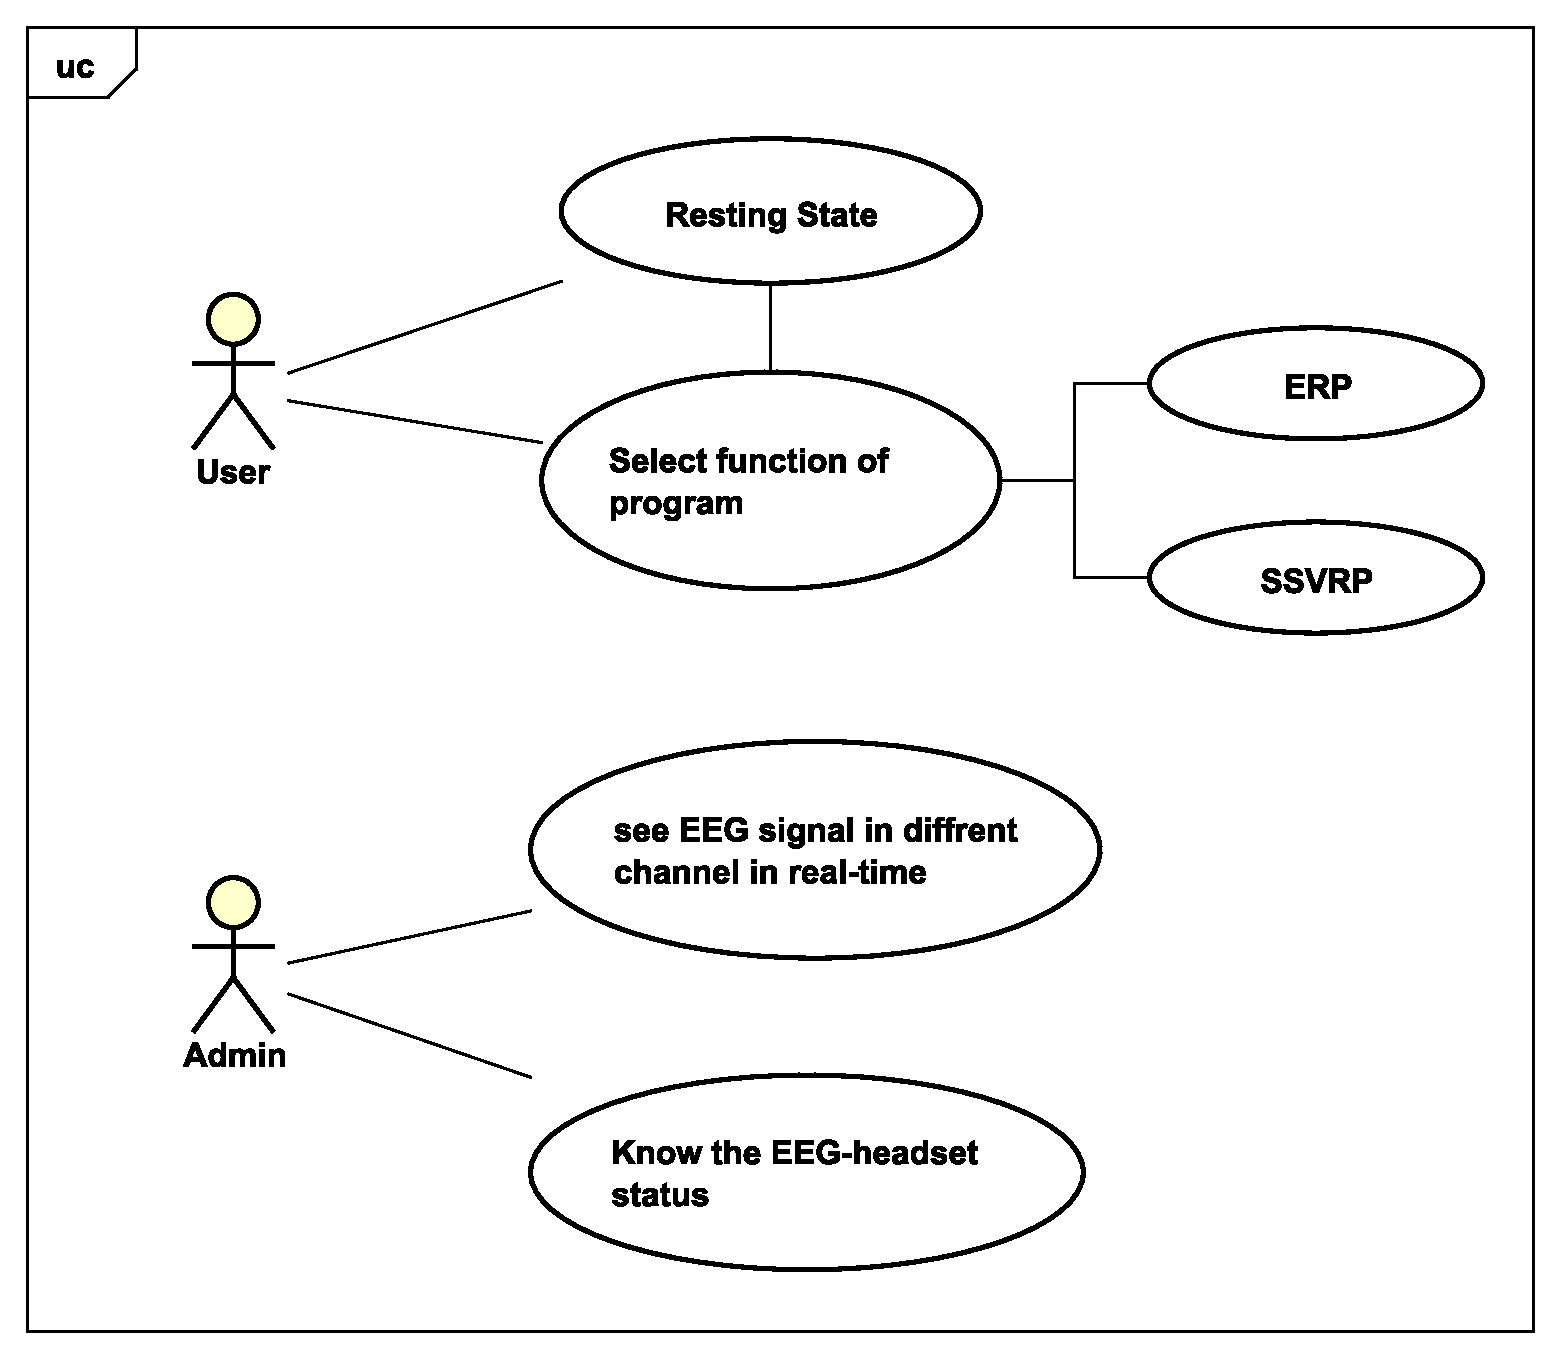
\includegraphics[scale=0.5]{chapter4/uc.pdf}
\caption{Use case diagram}
\end{figure}


\newpage{}


\subsection{Use case description for user and admin}
\begin{itemize}
	
\item \textbf{Expanded description of "Know the EEG-headset status
use case" }

\begin{description}
	\item [Use case:] Know the EEG-headset status 
	\item [Actor:] Admin 
	\item [Goal:] To make sure that the Emotiv headset will record EEG with
	the proper signal. 
	\item [Overview:] The admin will equip the Emotiv headset on the subject(user)
	head then observes the EEG-headset status to make sure that Emotiv
	headset will record SSVEP with the proper signal for the starting
	program for subject. 
	\item [Typical course of events:]~

	{
		\centering
	
		\begin{tabular}{| m{.47\linewidth} | m{.47\linewidth} |}
			
		\hline 
		\textbf{User} & \textbf{System}  \\
		\hline 
		1. Subject asks admin to access the system &   \\
		\hline 
		2. Subject is equipped the Emotiv headset by admin  &   \\
		\hline 
		& 3. The system returns the EEG-headset status (Green light) to admin \\
		\hline 
		4. Admin starts the program for subject & \\
		\hline 
		
		\end{tabular}
	}
	\item[Alternative:] The system returns poor EEG-headset status (red light) to admin and admin will move the EEG-headset to proper position (status – green light) before admin starts the program. 

\end{description}

\item \textbf{Expanded description of the "See EEG signal in different channel real-time" use case  }

\begin{description}
	\item [Use case:] See EEG signal in different channel real-time. 
	\item [Actor:] Admin 
	\item [Goal:] to observe the abnormal activities of brainwave and subject.  
	\item [Overview:] Admin must observe everything which take place in the chamber even the subject’s EEG to make sure that everything works fine.   
	\item [Typical course of events:]~
	
	{
		\centering
		
		\begin{tabular}{| m{.47\linewidth} | m{.47\linewidth} |}
			
			\hline 
			\textbf{User} & \textbf{System}  \\
			\hline 
			1. Subject asks admin to access the system &   \\
			\hline 
			2. Subject is equipped the Emotiv headset by admin  &   \\
			\hline 
			3. Subject gazes on the flickers of stimulus & \\
			\hline 
			4. Admin observes subject brainwave signal in different channel & \\
			\hline
			& 5. The system accepts the EEG of user \\
			\hline
			
		\end{tabular}
	}
	\item[Alternative:] Admin detects the abnormal magnitude EEG waveform then asks the subject to re-equip again.
	
\end{description}

\item \textbf{Expanded description of the "See peak of frequency domain" use case}
\begin{description}
	\item [Use case:] See peak of frequency domain 
	\item [Actor:] Admin 
	\item [Goal:] To let admin know that the system is in work in progress 
	\item [Overview:]The system allows the admin to see the peak of the frequency domain to let admin ensure that the system is calculating the subjects feature pattern while recording their SSVEP waveform. 
	\item [Typical course of events:]~
	
	{
		\centering
		
		\begin{tabular}{| m{.47\linewidth} | m{.47\linewidth} |}
			
			\hline 
			\textbf{User} & \textbf{System}  \\
			\hline 
			1. Subject asks admin to access the system &   \\
			\hline 
			2. Subject is equipped the Emotiv headset by admin  &   \\
			\hline 
			3. Subject gazes on the flickers of stimulus & \\
			\hline 
			& 4. The system will calculate the feature pattern and show the result of calculation to admin  \\
			\hline
			5. Admin observes the subject’s peak frequency domain & \\
			\hline
			
		\end{tabular}
	}
	
\end{description}

\item \textbf{Expanded description of the "Resting state" use case }
\begin{description}
	\item [Previous cases:] -
	\item [Use case:] Resting state
	\item [Actor:] User  
	\item [Goal:] To obtain the EEG of user in general state. 
	\item [Overview:] This is a step that every user must pass this step to control the program in next step. The EEG of the user that be obtained in this step we use it like a baseline. 
	\item [Typical course of events:]~
	
	{
		\centering
		
		\begin{tabular}{| m{.47\linewidth} | m{.47\linewidth} |}
			
			\hline 
			\textbf{User} & \textbf{System}  \\
			\hline 
			1. Subject asks admin to access the system. &   \\
			\hline 
			2. Subject is equipped the Emotive headset bu admin   &   \\
			\hline 
			& 3. The System will show the status of Emotiv headset \\
			\hline 
			4. Admins will tell Subject about Emotiv's status is good &  \\
			\hline
			5. Subject gazes on the flickers of stimulus &  \\
			\hline
			& 6. The system will obtain the EEG of subject to use in next step\\
			\hline
			
		\end{tabular}
	}
	
\end{description}

\item \textbf{Expanded description of the "Select the menu program" use case }
\begin{description}
	\item [Previous cases:] Resting state
	\item [Use case:] Select the menu program
	\item [Actor:] User  
	\item [Goal:] To be granted select the menu program from the system. 
	\item [Overview:] This is also the step that every user who want to grant select the menu to control the program. The EEG of the subject has to match to the EEG that subject is recorded the baseline’s EEG.
	\item [Typical course of events:]~
	
	{
		\centering
		
		\begin{tabular}{| m{.47\linewidth} | m{.47\linewidth} |}
			
			\hline 
			\textbf{User} & \textbf{System}  \\
			\hline 
			1. Subject passed the register process &   \\
			\hline 
			2. Subject gazes on the flickers of stimulus   &   \\
			\hline 
			& 3. The system will record the subject’s EEG \\
			\hline 
			& 4. The system will match the EEG with the EEG of subject’s baseline  \\
			\hline
			& 5. The system will determine what menu that user want to select \\
			\hline
			& 6. The system will select the menu program\\
			\hline
			
		\end{tabular}
	}
	
\end{description}


\end{itemize}


\section{Activity Diagram}


\subsection{Activity diagram of resting state}

\begin{figure}[ht]
\centering 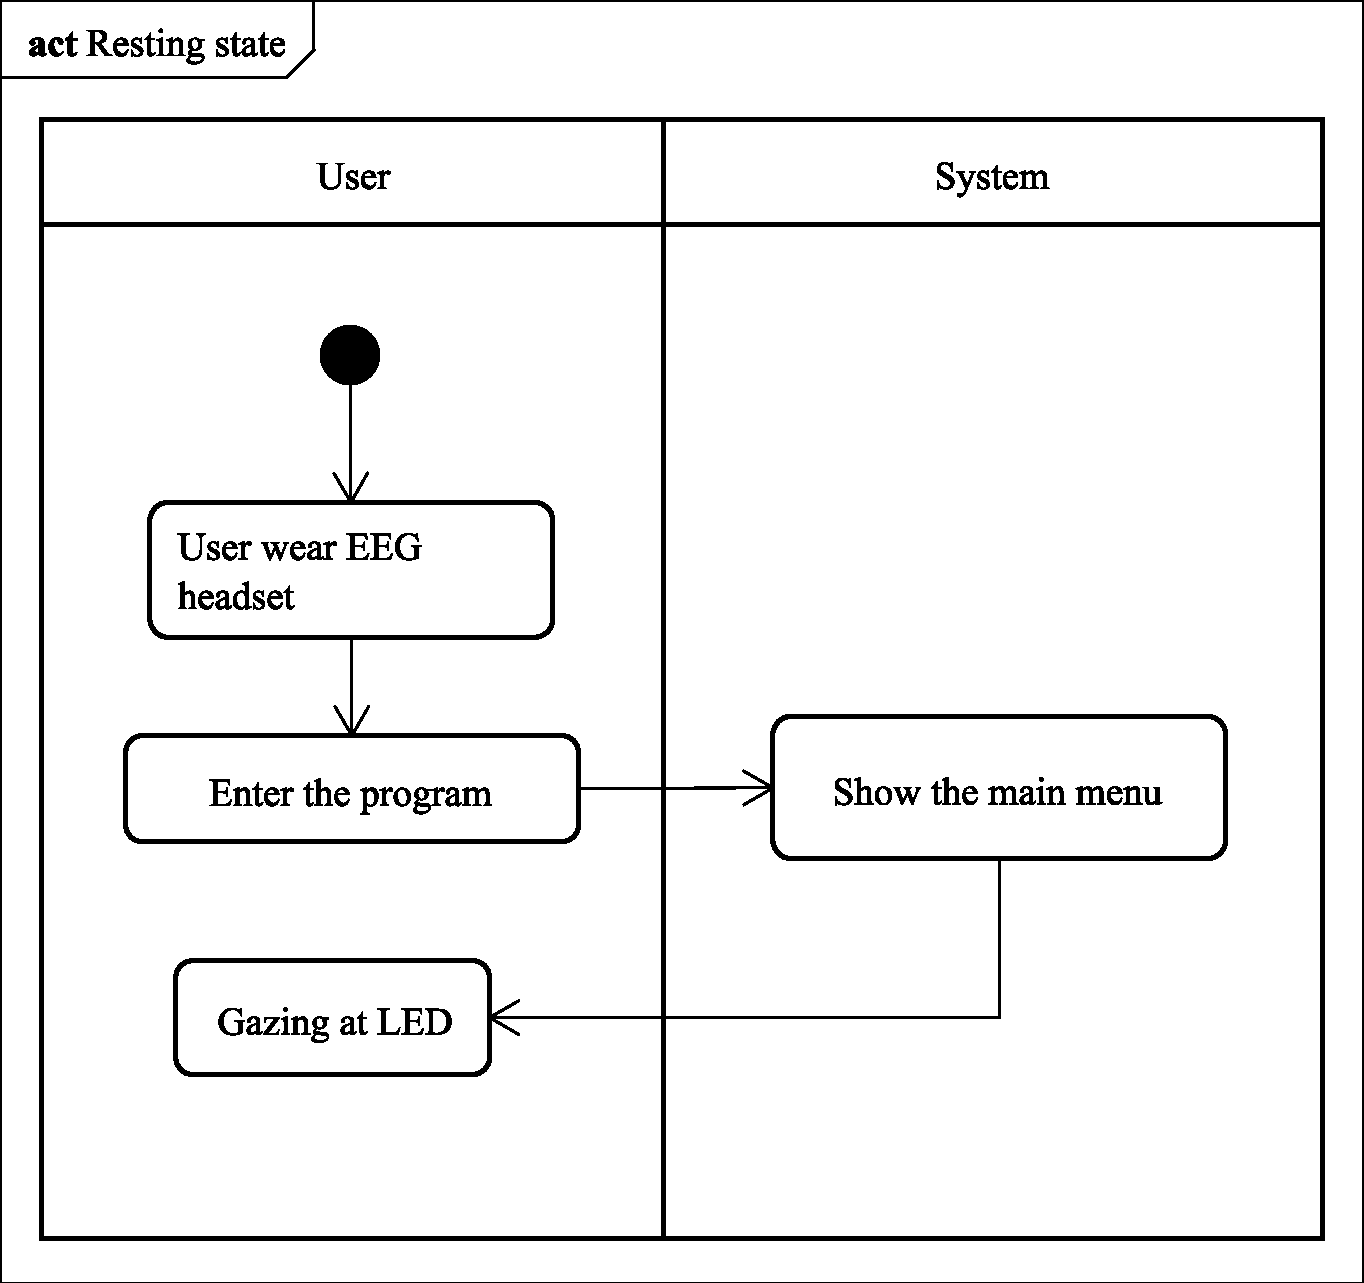
\includegraphics[scale=0.295]{chapter4/Rest.pdf}
\caption{Activity diagram of resting state}
\end{figure}



\subsection{Activity diagram of ERP}

\begin{figure}[ht]
\centering 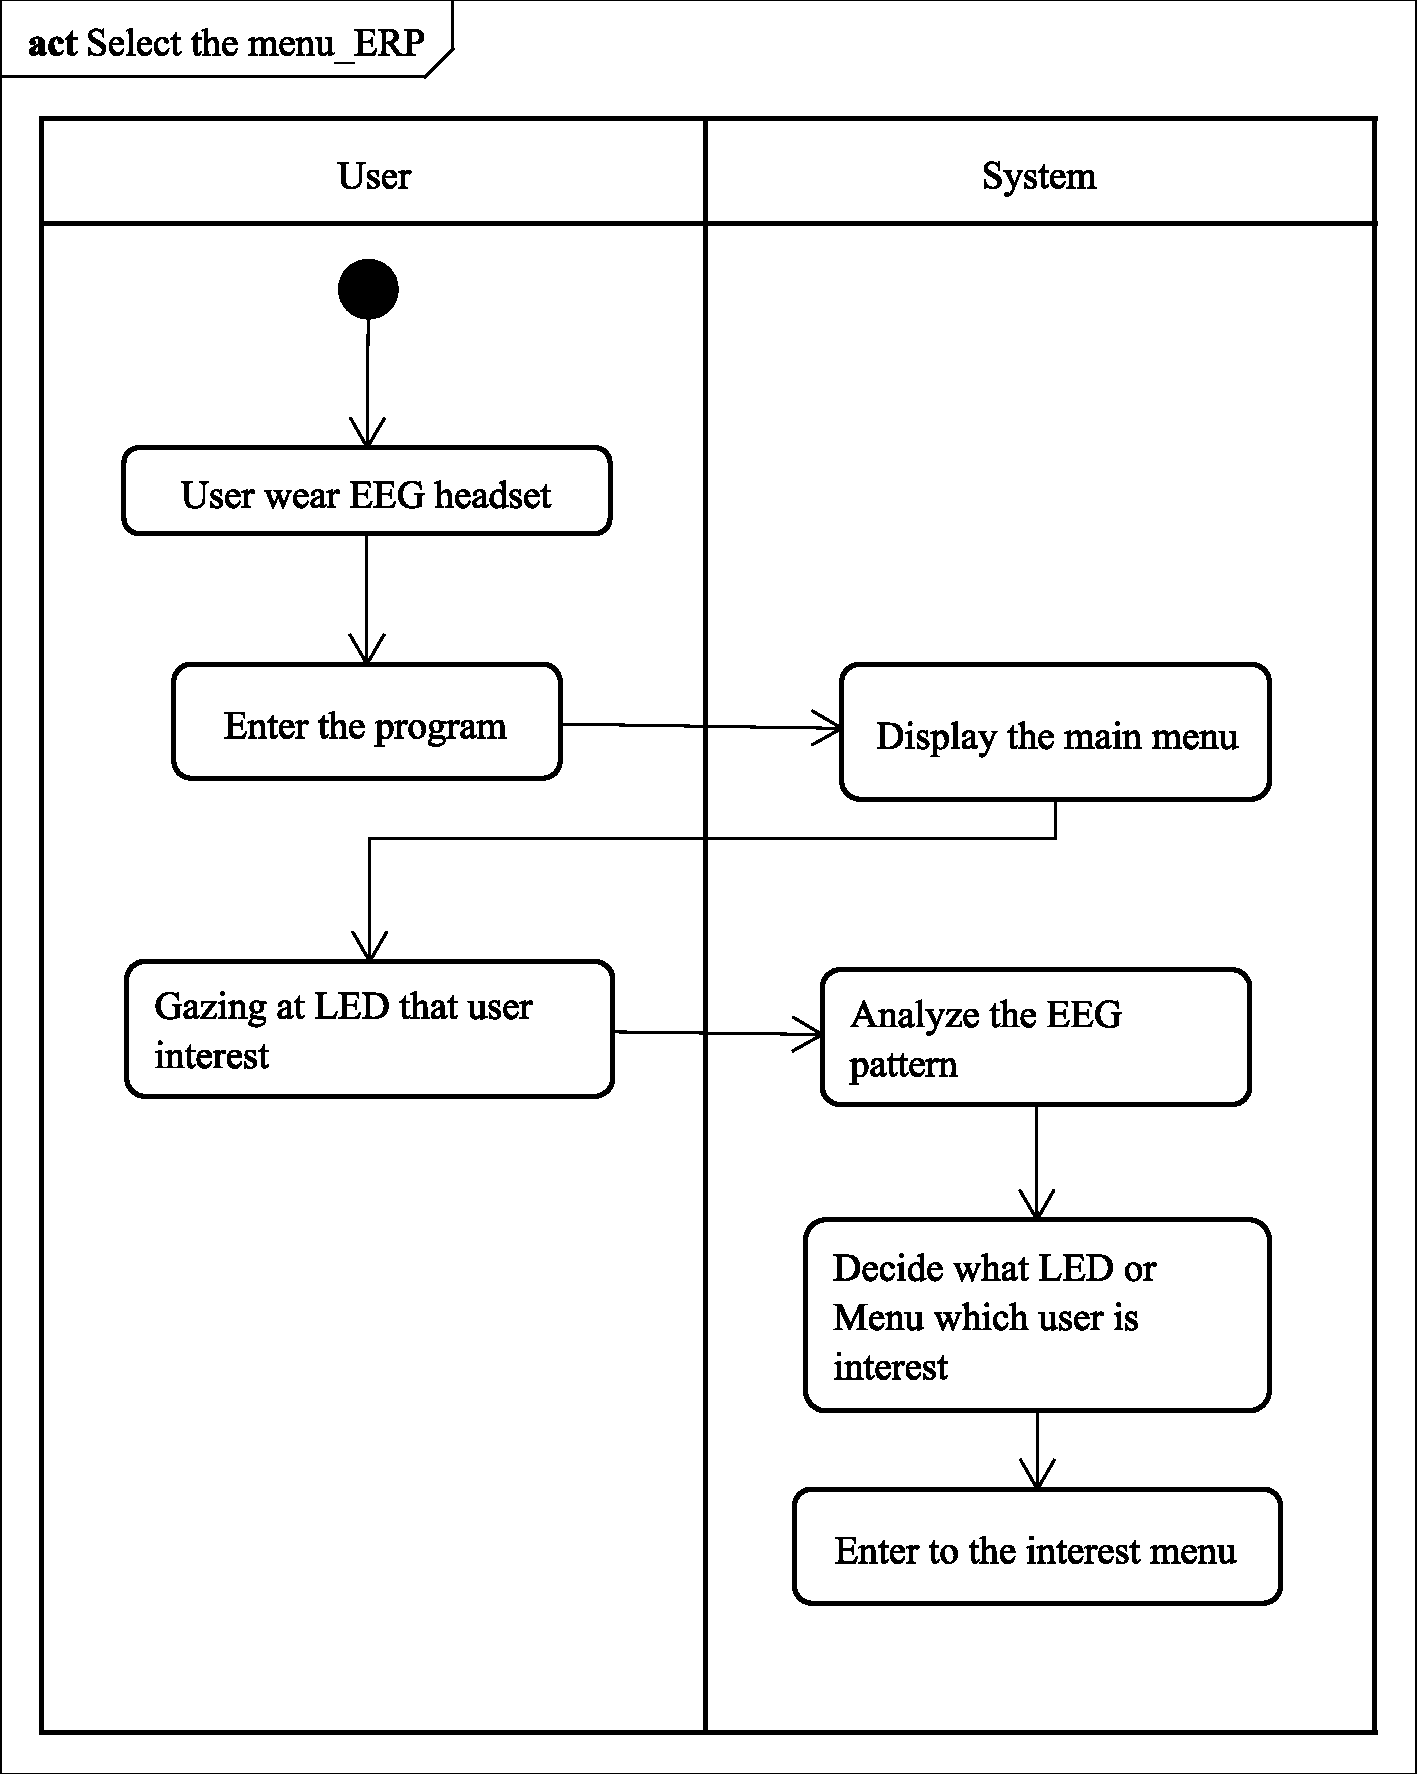
\includegraphics[scale=0.295]{chapter4/av_ERP.pdf}
\caption{Activity diagram of ERP}
\end{figure}


\newpage{}

\subsection{Activity diagram of SSVEP}

\begin{figure}[ht]
\centering 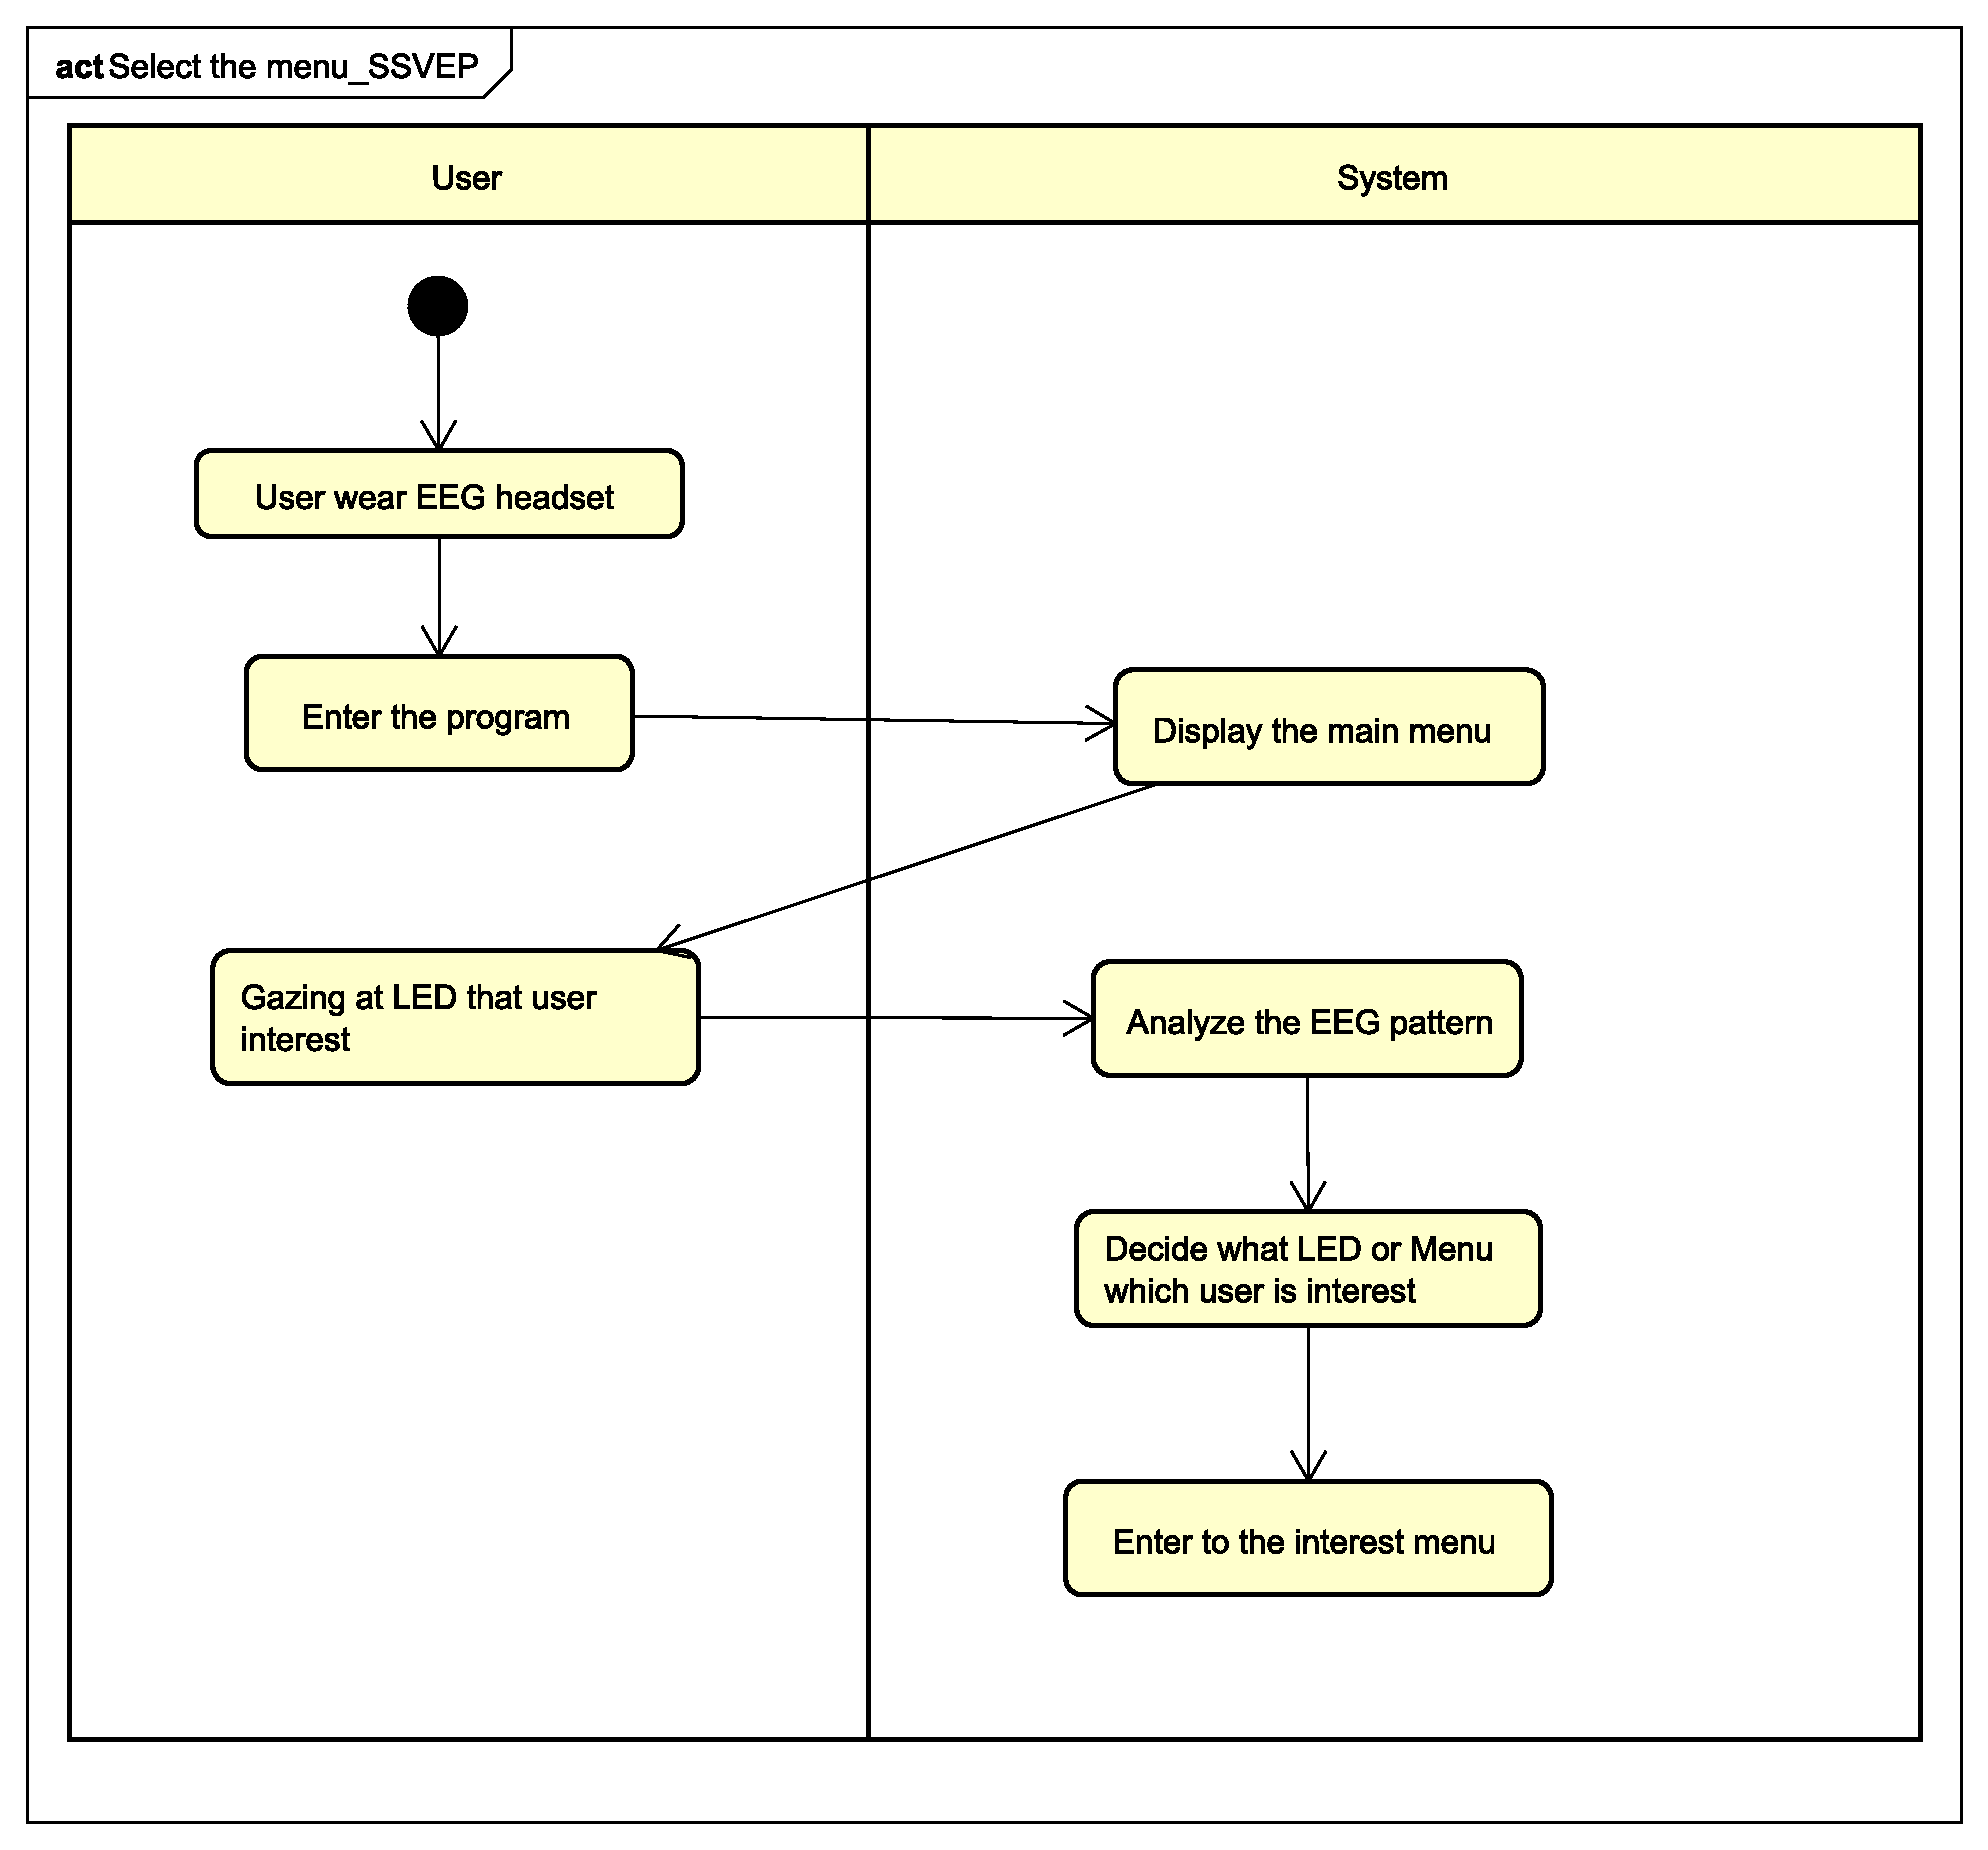
\includegraphics[scale=0.295]{chapter4/av_SSVEP.pdf}
\caption{Activity diagram of SSVEP}
\end{figure}

